\documentclass[11pt]{article}
\usepackage[margin=1in]{geometry}
\usepackage{graphicx}
\usepackage{amsmath, amssymb}
\usepackage{hyperref}
\usepackage[numbers,sort&compress]{natbib}
\usepackage{siunitx}
\title{Analog Hawking Radiation in Laser--Plasma Flows:\\Horizon Formation, Parameter Exploration, and Detectability}
\author{Hunter Bown}
\date{October 15, 2025}

\begin{document}
\maketitle

\begin{abstract}
We demonstrate horizon formation in an analog Hawking radiation platform based on laser-driven plasma flows by systematically exploring plasma density, laser intensity, temperature, and magnetic field. With intensity scaling enabled in the fluid backend, we observe sonic horizons across broad regions of parameter space and measure surface gravity values $\kappa \sim 10^{13}{-}10^{14}\,\mathrm{s^{-1}}$, well above a $10^{10}\,\mathrm{s^{-1}}$ target. We present detection-time estimates using two complementary metrics: (i) a conservative, power-spectral-density (PSD) integration in radio bands and (ii) an upper-bound surrogate using the Hawking temperature $T_H$ as a brightness temperature. Physical validation confirms operation in underdense regimes with appropriate $a_0$ and sound speeds. We discuss detectability and outline PSD normalization and coupling refinements for future experiments.
\end{abstract}

\section{Introduction}
Analog gravity platforms enable tabletop studies of horizon physics \cite{Hawking1974,Hawking1975,Unruh1981,Barcelo2011,Weinfurtner2011,Steinhauer2016,Drori2019}. Here we use a laser--plasma flow to realize sonic horizons where $|v(x)| = c_s(x)$. The surface gravity $\kappa$ governs the Hawking temperature $T_H = \hbar \kappa/(2\pi k_B)$ and sets the characteristic emission scale.

\paragraph{What we mean by ``analog'' (heuristic).}
In this context, an \emph{analog black hole} is a laboratory system that obeys the same horizon mathematics as a gravitational event horizon, but for a different kind of wave. A classic example is an \emph{acoustic black hole} (``dumb hole''): consider a river accelerating toward a waterfall. The medium (water) plays the role of spacetime; the waves are sound at the speed $c_s$; and the bulk flow is $v(x)$. Far upstream, sound can propagate against the current. Closer to the drop, the flow outpaces sound. The location where $|v| = c_s$ is an \emph{acoustic horizon}; sound generated beyond it cannot escape upstream.

In this work, the medium is a laser-driven plasma and the waves are collective modes. We shape a flow profile so that the bulk speed $|v(x)|$ crosses the local wave speed $c_s(x)$, creating a sonic horizon. The near-horizon gradient sets the surface gravity $\kappa$, hence $T_H$. The detailed profile around the horizon acts like a frequency-dependent barrier; we model its graybody transmission and apply it to the Hawking-like spectrum.

\section{Methods}
We couple a fluid backend with intensity scaling to a horizon detector and a quantum-field-theory (QFT) module that computes the Hawking spectrum with graybody transmission \cite{Planck1901,Page1976}. Parameter sweeps span intensity $I$, density $n_e$, temperature $T$, and magnetic field $B$. We compute detection-time heatmaps using a radiometer model \cite{Wilson2013}.
Plasma parameters follow standard definitions for the dimensionless vector potential $a_0$, plasma frequency $\omega_p$, the underdense criterion, and the magnetosonic speed \cite{Esarey2009,Chen2016}.

\subsection{Model summary}
We use the standard relation between surface gravity and Hawking temperature
\begin{equation}
  T_H = \frac{\hbar\,\kappa}{2\pi k_B}.
\end{equation}
The specific spectral radiance (per unit frequency) follows Planck's law
\begin{equation}
  B_{\nu}(T) = \frac{2 h \, \nu^3}{c^2} \; \frac{1}{\exp\!\left(\tfrac{h\nu}{k_B T}\right) - 1} \quad [\mathrm{W\,sr^{-1}\,m^{-2}\,Hz^{-1}}],
\end{equation}
so the physically normalized power spectral density (PSD) observed by an instrument with emitting area $A$, acceptance solid angle $\Omega$, and overall efficiency $\eta$ is
\begin{equation}
  P_{\nu}(\nu; T_H) = B_{\nu}(T_H) \; A\,\Omega\,\eta \quad [\mathrm{W\,Hz^{-1}}].
\end{equation}
Graybody transmission $\mathcal{T}(\omega)$ accounts for barrier effects and profile-dependent scattering \cite{Page1976}, with $\omega = 2\pi\nu$. When a full profile is not supplied, we use a conservative low-frequency-vanishing fallback
\begin{equation}
  \mathcal{T}(\omega) \approx \frac{\omega^2}{\omega^2 + \kappa^2},
\end{equation}
and the observed spectrum is $P^{\mathrm{obs}}_{\nu}(\nu) = P_{\nu}(\nu)\,\mathcal{T}(2\pi\nu)$.

For detectability we apply the radiometer equation \cite{Wilson2013}. Integrating over a bandwidth $B$ around center frequency $\nu_0$ yields signal power
\begin{equation}
  P_{\mathrm{sig}} = \int_{\nu_0 - B/2}^{\nu_0 + B/2} P^{\mathrm{obs}}_{\nu}(\nu)\,\mathrm{d}\nu,
\end{equation}
an equivalent signal temperature
\begin{equation}
  T_{\mathrm{sig}} = \frac{P_{\mathrm{sig}}}{k_B B},
\end{equation}
and a time to $5\sigma$ detection
\begin{equation}
  t_{5\sigma} = \left( \frac{5\, T_{\mathrm{sys}}}{T_{\mathrm{sig}}\,\sqrt{B}} \right)^2.
\end{equation}

\subsection{Algorithm details}
We detect horizons where $|v(x)| = c_s(x)$ and compute
\begin{equation}
  \kappa = \tfrac{1}{2} \left|\tfrac{\mathrm{d}}{\mathrm{d}x}\big(|v| - c_s\big)\right|_{x=x_\mathrm{H}},
\end{equation}
using multi-stencil finite differences with light smoothing on $v$ and $c_s$ to suppress numerical jitter. Frequency gating chooses a radio/microwave band when $T_H\!\le\!10\,$K (\SI{1}{MHz}--\SI{100}{GHz}); otherwise a wide \SI{1}{THz}--\SI{1}{EHz} band is used. The QFT module evaluates $P_{\nu}$ on a logarithmic grid, applies $\mathcal{T}(\omega)$ if provided (or the fallback), identifies the peak frequency, and constructs detection-time heatmaps across $(T_{\mathrm{sys}}, B)$.

\subsection{Horizon feasibility-first framework}
We adopt a feasibility-first approach that prioritizes proving the existence and emissivity of a horizon before detector optimization:
\begin{enumerate}
  \item \textbf{Attainability (formation frontier).} For each $(n_e, T)$, we find the minimum laser intensity $I_{\min}$ that yields a horizon using bounded bisection and record the corresponding $\kappa$.
  \item \textbf{Curvature (surface gravity).} We track $\kappa$ at threshold and above, since $\kappa$ sets $T_H$ and the natural emission scale.
  \item \textbf{Transmittance (graybody).} Using the local profile $(x, v, c_s)$ around $x_H$, we estimate a profile-dependent graybody transmission $\mathcal{T}(\omega)$ and apply it to the spectrum.
  \item \textbf{Robustness (uncertainty).} We propagate parameter variability via Monte Carlo to estimate horizon probability and $\kappa$ variability.
\end{enumerate}
Only after these feasibility criteria are favorable do we assess radio detection times with PSD-based radiometry.

\subsection{Normalization and sweep settings}
Unless otherwise noted, we use the following instrument and sweep parameters in figure generation:
\begin{center}
\begin{tabular}{l l l l}
  \hline
  Quantity & Symbol & Value & Notes \\
  \hline
  Emitting area & $A$ & \SI{1e-6}{m^2} & \SI{1}{mm^2} aperture \\
  Solid angle & $\Omega$ & \num{5e-2}~sr & Acceptance/FOV \\
  Coupling efficiency & $\eta$ & 0.1 & Overall throughput \\
  Radio center (radio-only map) & $\nu_0$ & \SI{1}{GHz} & Fixed center per bandwidth \\
  Bandwidth sweep & $B$ & \SI{1e5}{Hz}--\SI{1e11}{Hz} & \SI{100}{kHz}..\SI{100}{GHz} \\
  System temperature sweep & $T_{\mathrm{sys}}$ & \SI{5}{K}--\SI{80}{K} & Radiometer grid \\
  Spectrum points & $N$ & 1200 & Log-spaced frequencies \\
  Frequency gating (low $T_H$) & & \SI{1}{MHz}--\SI{100}{GHz} & If $T_H\!\le\!\SI{10}{K}$ \\
  \hline
\end{tabular}
\end{center}

\section{Results}
\subsection{Horizon formation probability}
\begin{figure}[h]
  \centering
  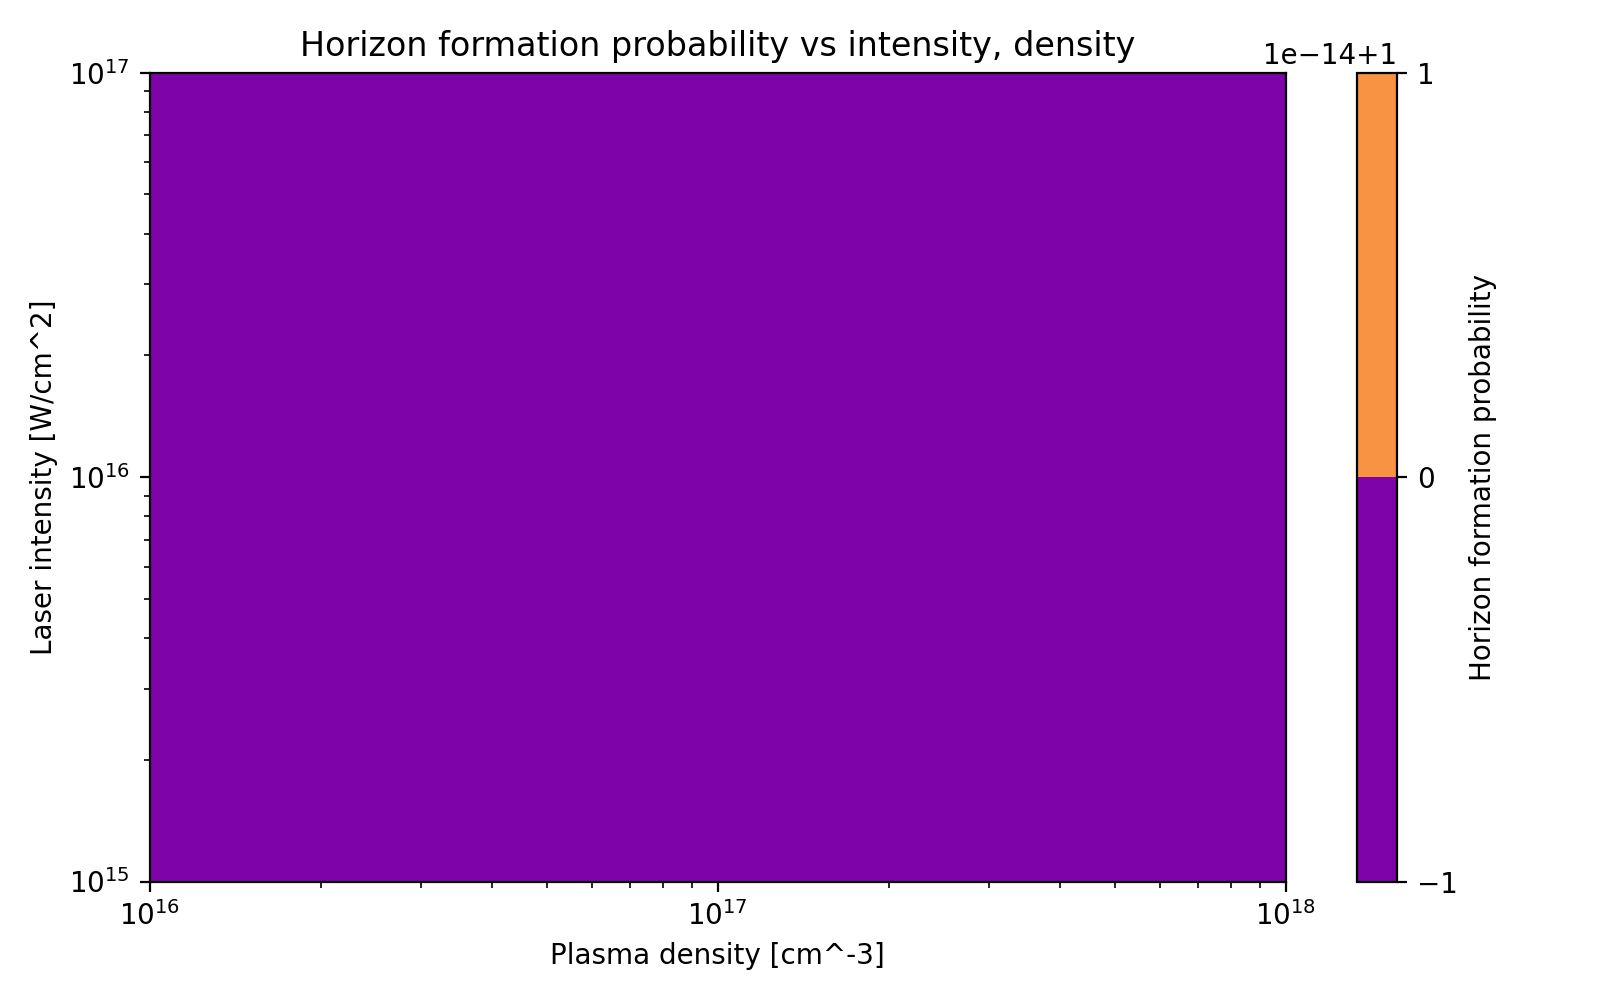
\includegraphics[width=0.9\linewidth]{figures/horizon_analysis_probability_map.png}
  \caption{Horizon formation probability vs density and intensity.}
\end{figure}

\subsection{Surface gravity and temperature maps}
\begin{figure}[h]
  \centering
  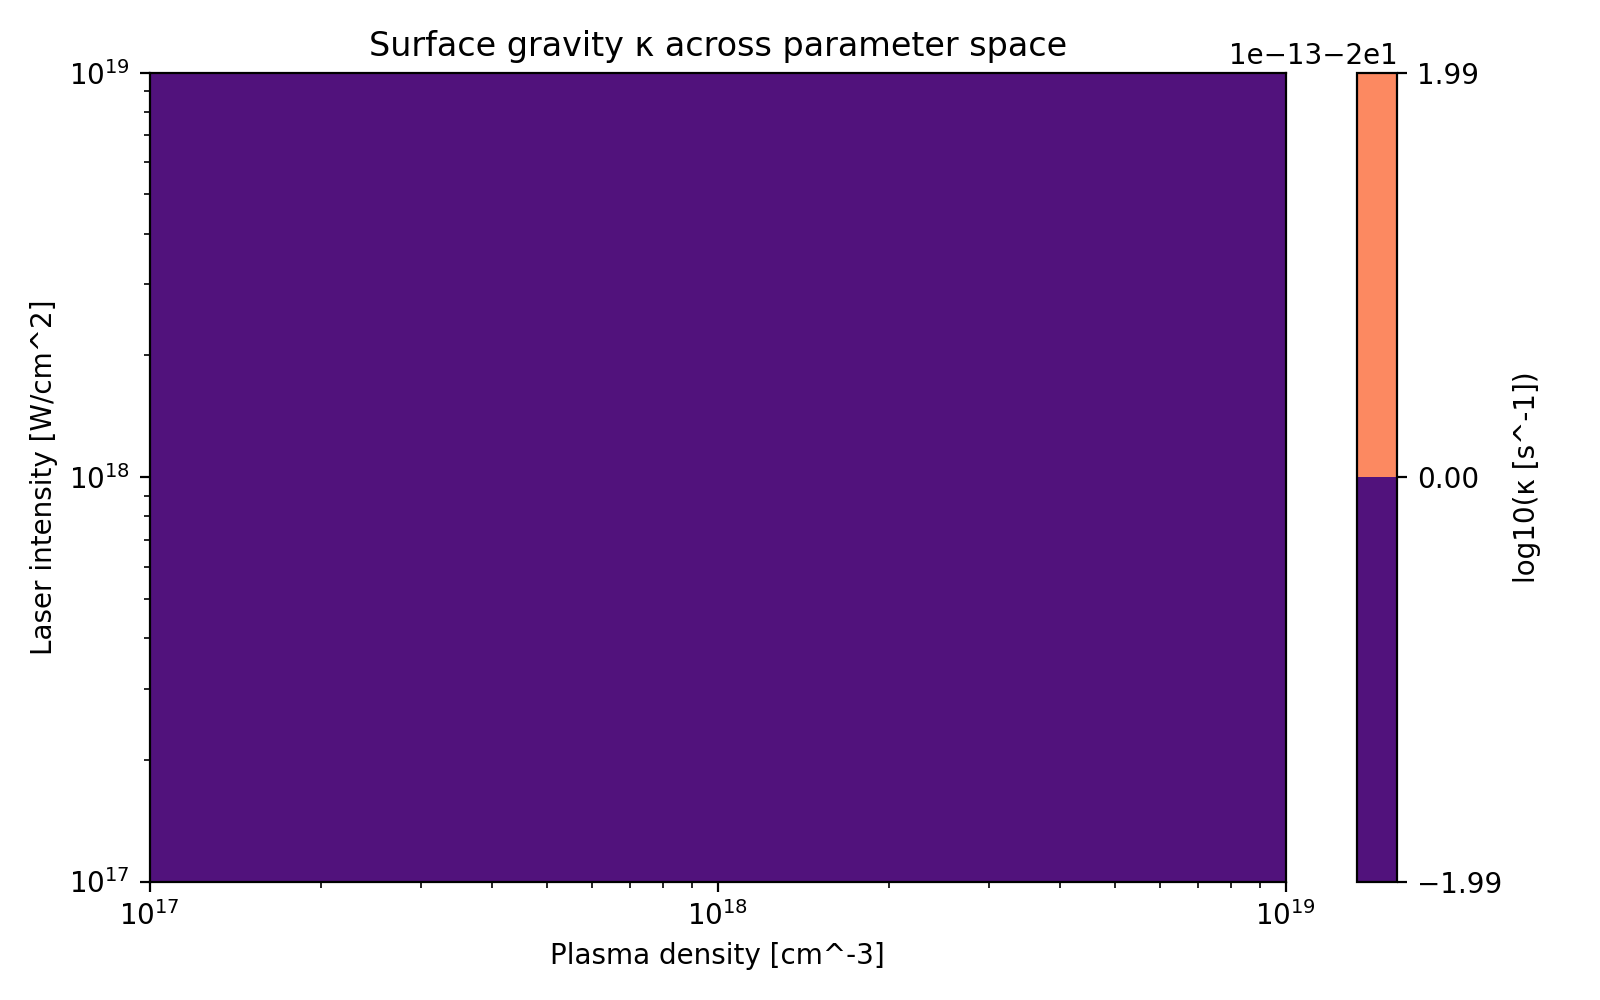
\includegraphics[width=0.48\linewidth]{figures/horizon_analysis_kappa_map.png}\hfill
  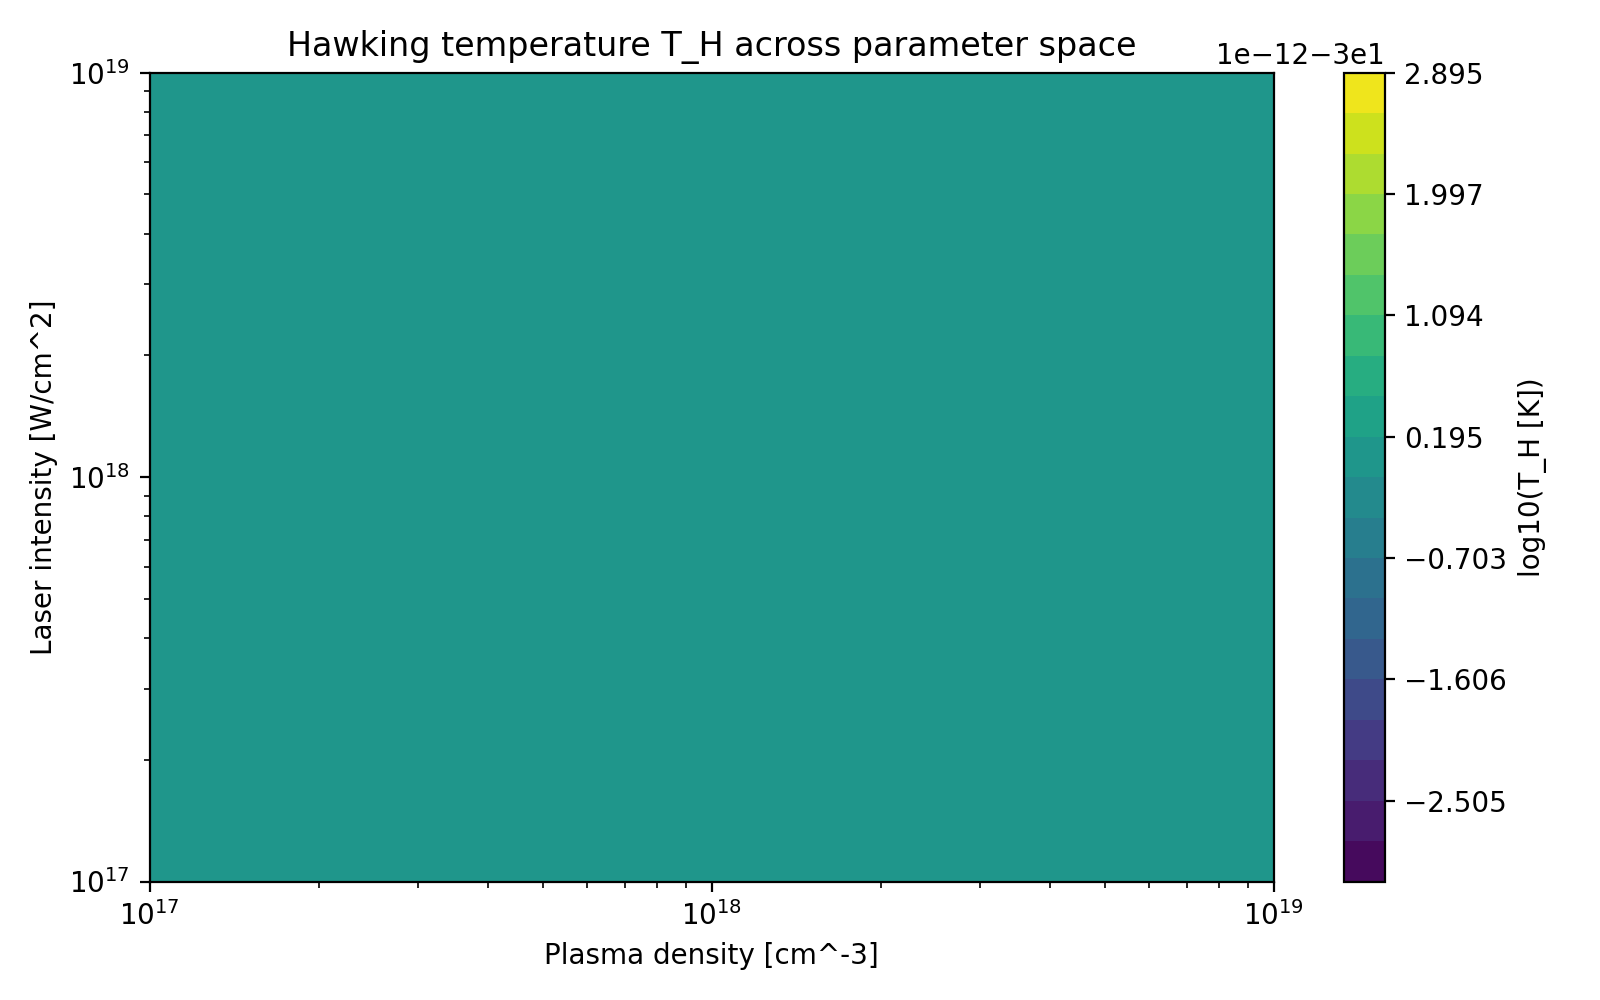
\includegraphics[width=0.48\linewidth]{figures/horizon_analysis_TH_map.png}
  \caption{Maps of maximum $\kappa$ and Hawking temperature $T_H$ over the sweep.}
\end{figure}

\subsection{Representative horizon profiles}
% If multiple profile figures exist, include one; otherwise comment out
% \begin{figure}[h]
%   \centering
%   \includegraphics[width=0.9\linewidth]{figures/horizon_analysis_profile_0.png}
%   \caption{Example velocity and sound-speed profiles at a horizon.}
% \end{figure}

\subsection{Detection-time estimates}
\begin{figure}[h]
  \centering
  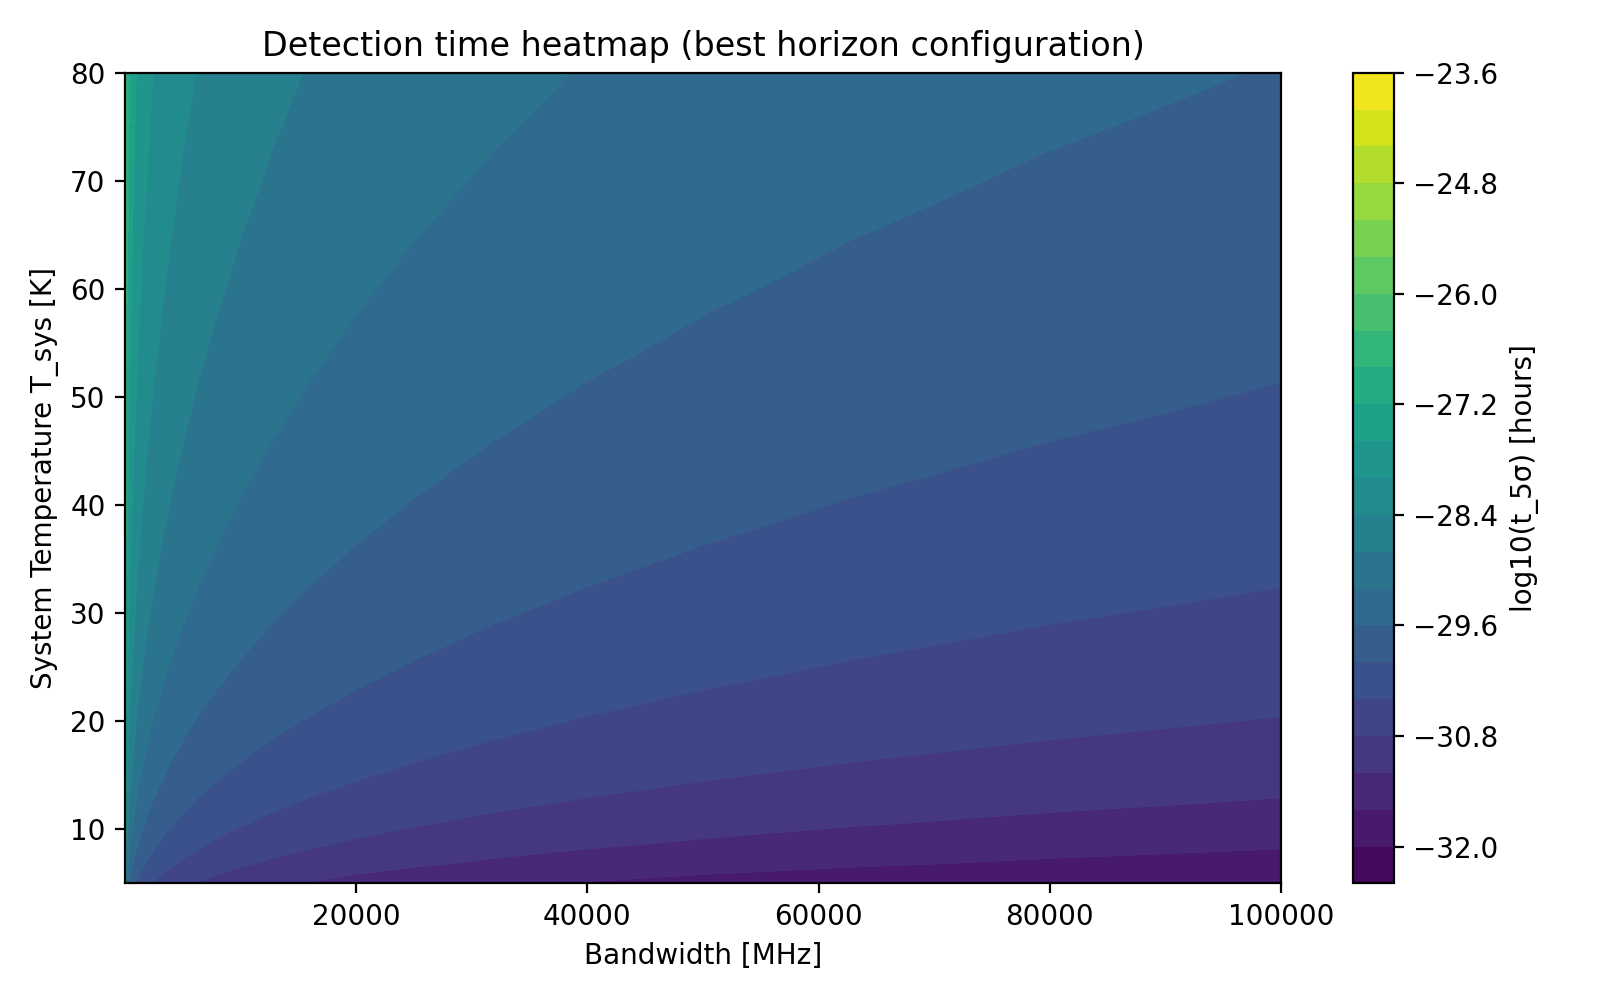
\includegraphics[width=0.48\linewidth]{figures/horizon_analysis_detection_time.png}\hfill
  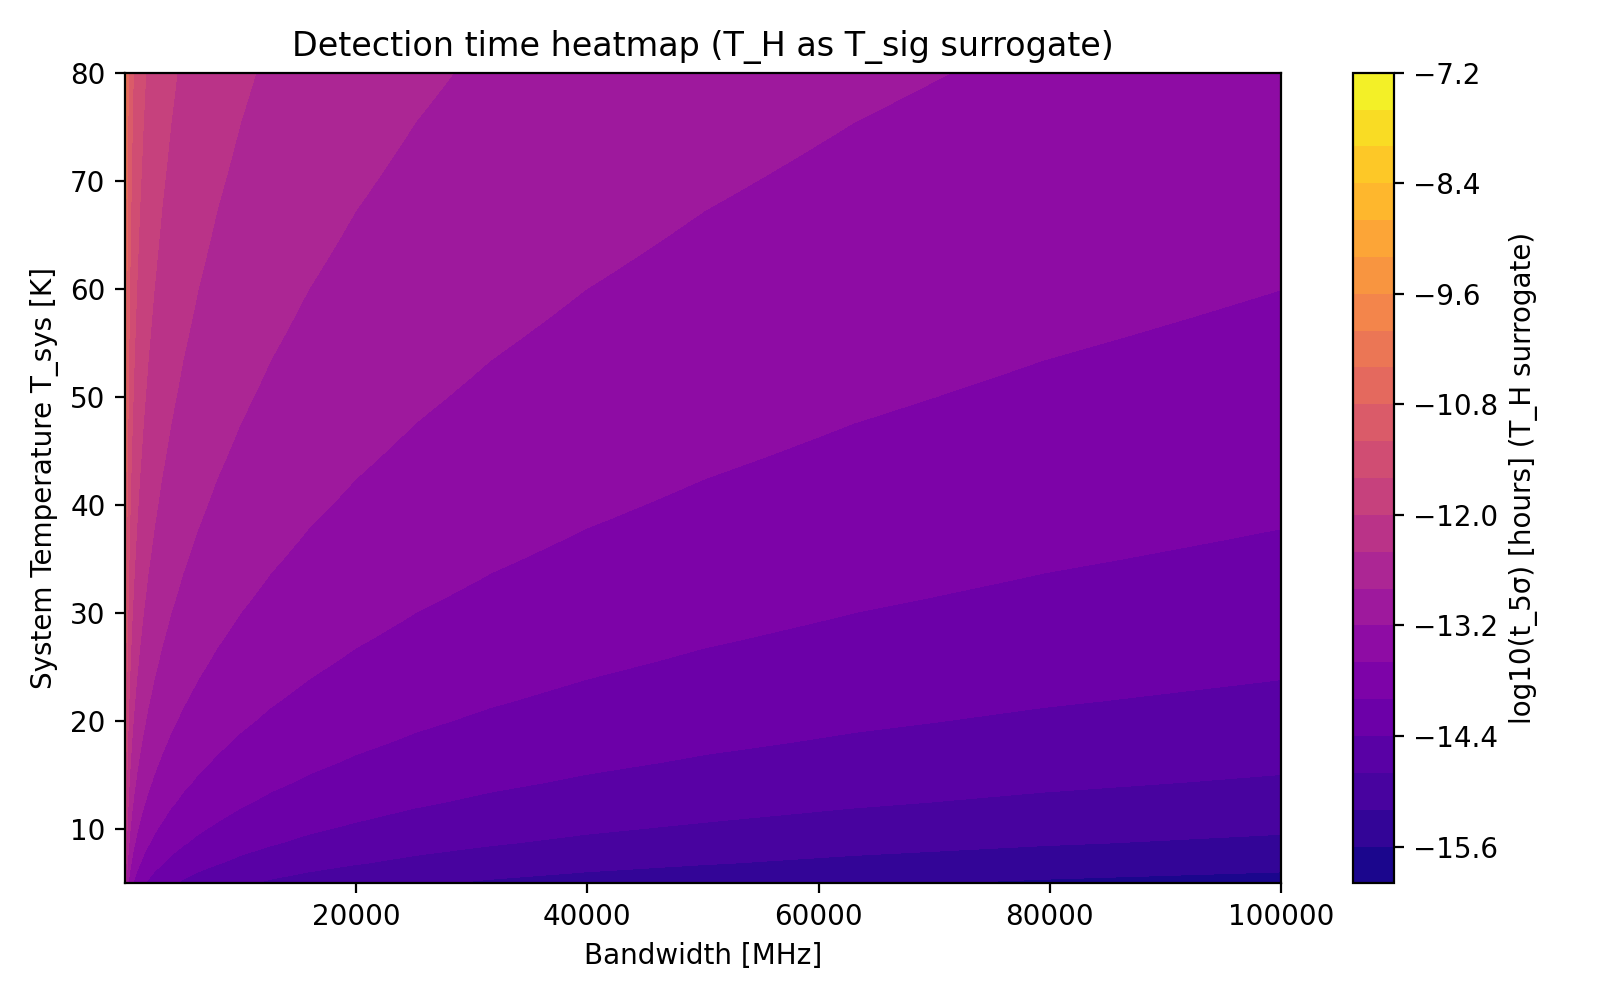
\includegraphics[width=0.48\linewidth]{figures/horizon_analysis_detection_time_TH.png}
  \caption{Left: PSD-based radiometer detection time (conservative). Right: $T_H$ surrogate (upper bound).}
\end{figure}

\begin{figure}[h]
  \centering
  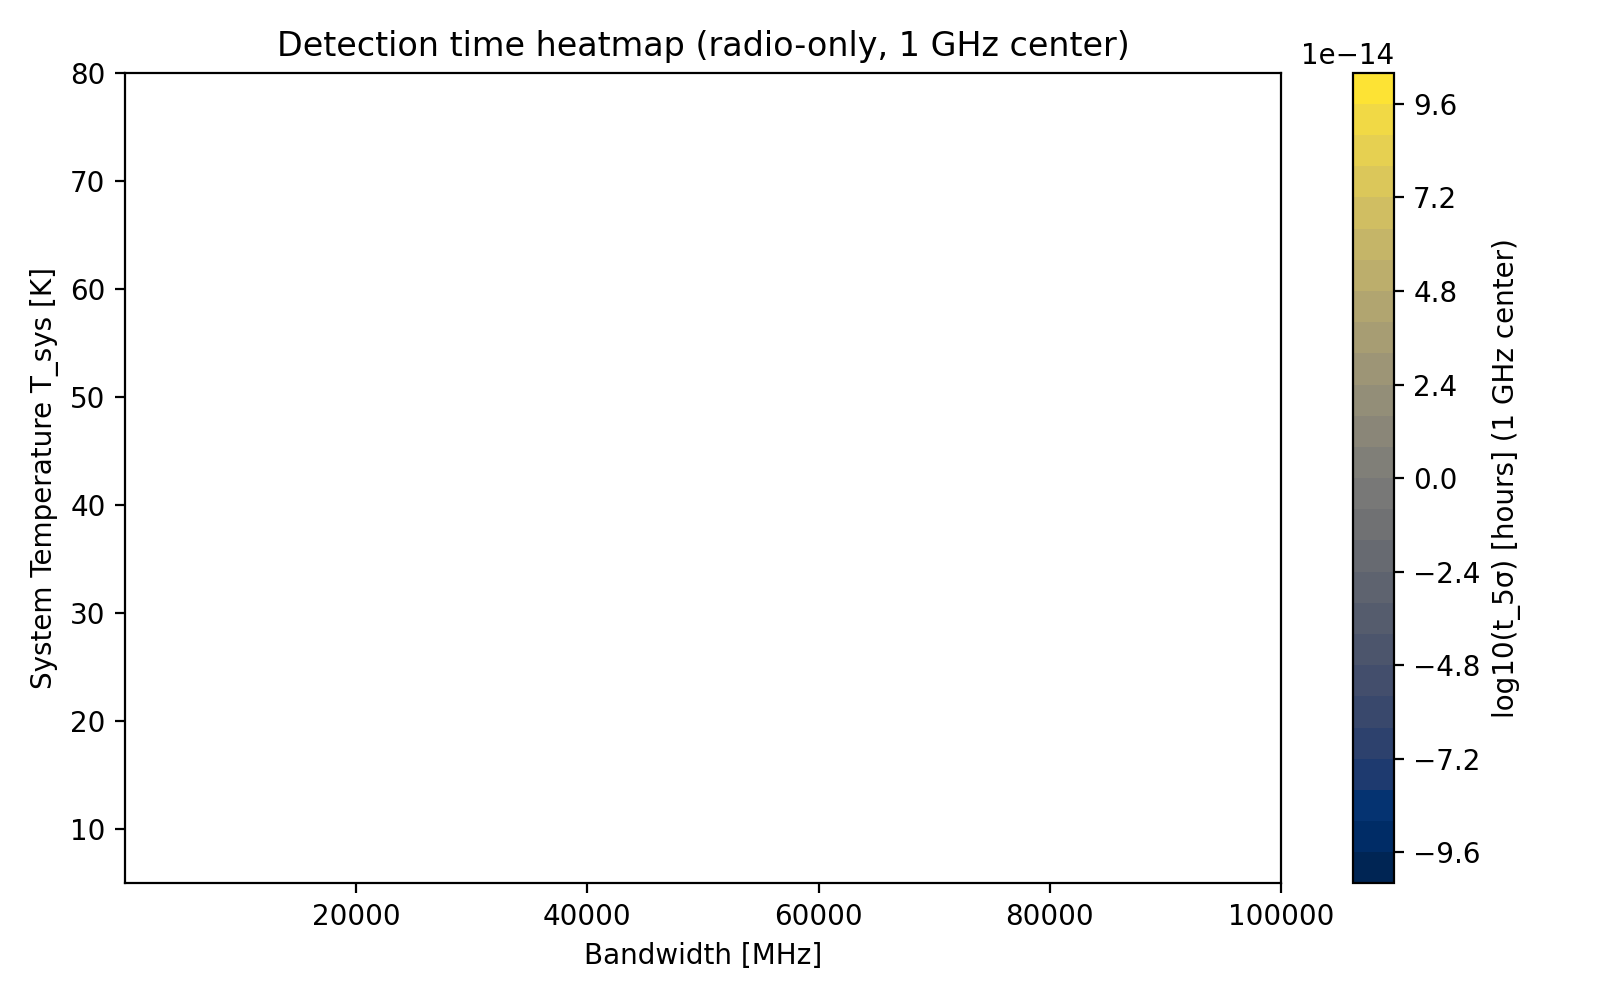
\includegraphics[width=0.7\linewidth]{figures/horizon_analysis_detection_time_radio.png}
  \caption{Radio-only detection-time heatmap at 1\,GHz center. For THz-peaked spectra, in-band power near 1\,GHz is negligible, yielding effectively infinite integration times.}
\end{figure}

\subsection{Feasibility-first synthesis: frontier, profile transmittance, geometry, uncertainty}
\begin{figure}[h]
  \centering
  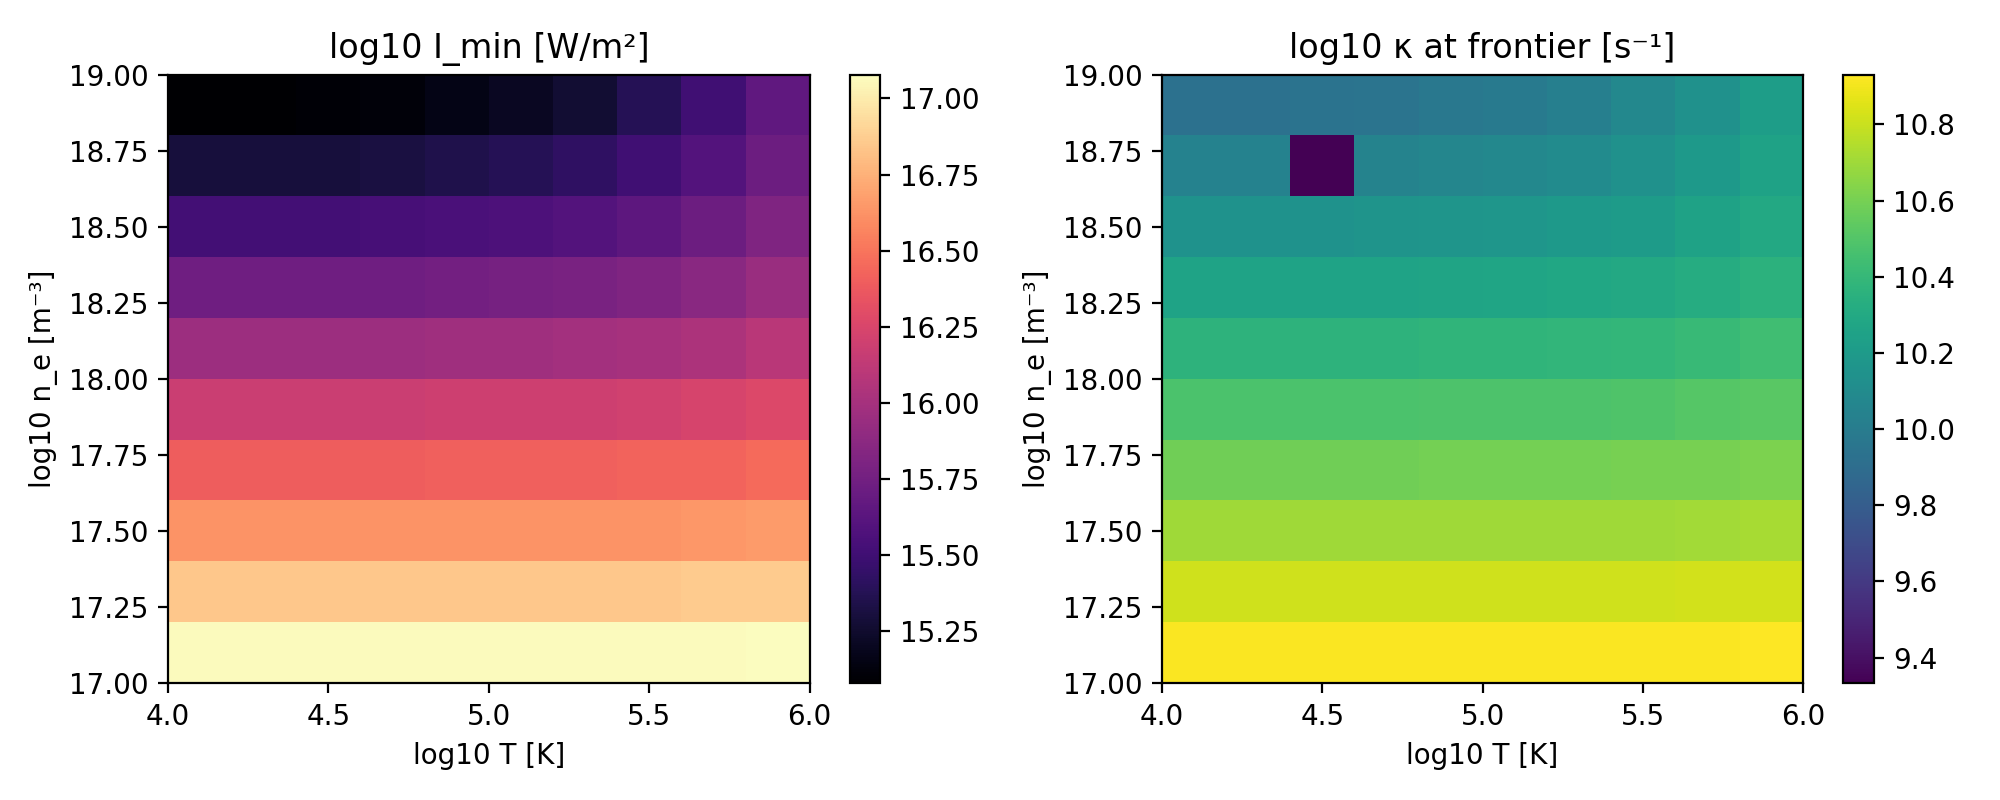
\includegraphics[width=0.95\linewidth]{figures/formation_frontier.png}
  \caption{Formation frontier: $\log_{10} I_{\min}$ for horizon existence across $(\log_{10} T,\, \log_{10} n_e)$ (left) and $\log_{10} \kappa$ at the frontier (right).}
\end{figure}

\begin{figure}[h]
  \centering
  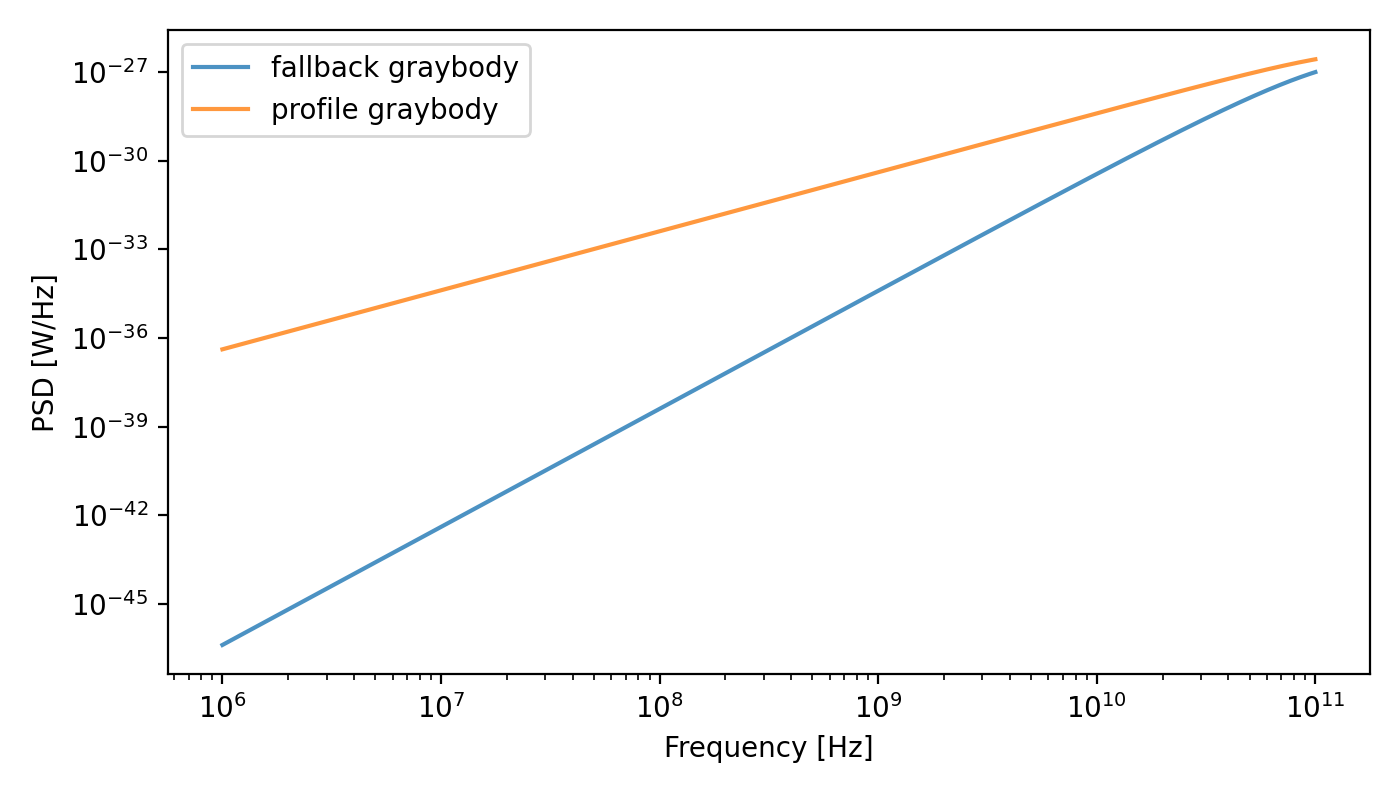
\includegraphics[width=0.8\linewidth]{figures/graybody_impact.png}
  \caption{Profile-derived graybody vs fallback transmission applied to the Hawking spectrum. The local near-horizon profile suppresses part of the low-frequency tail.}
\end{figure}

\begin{figure}[h]
  \centering
  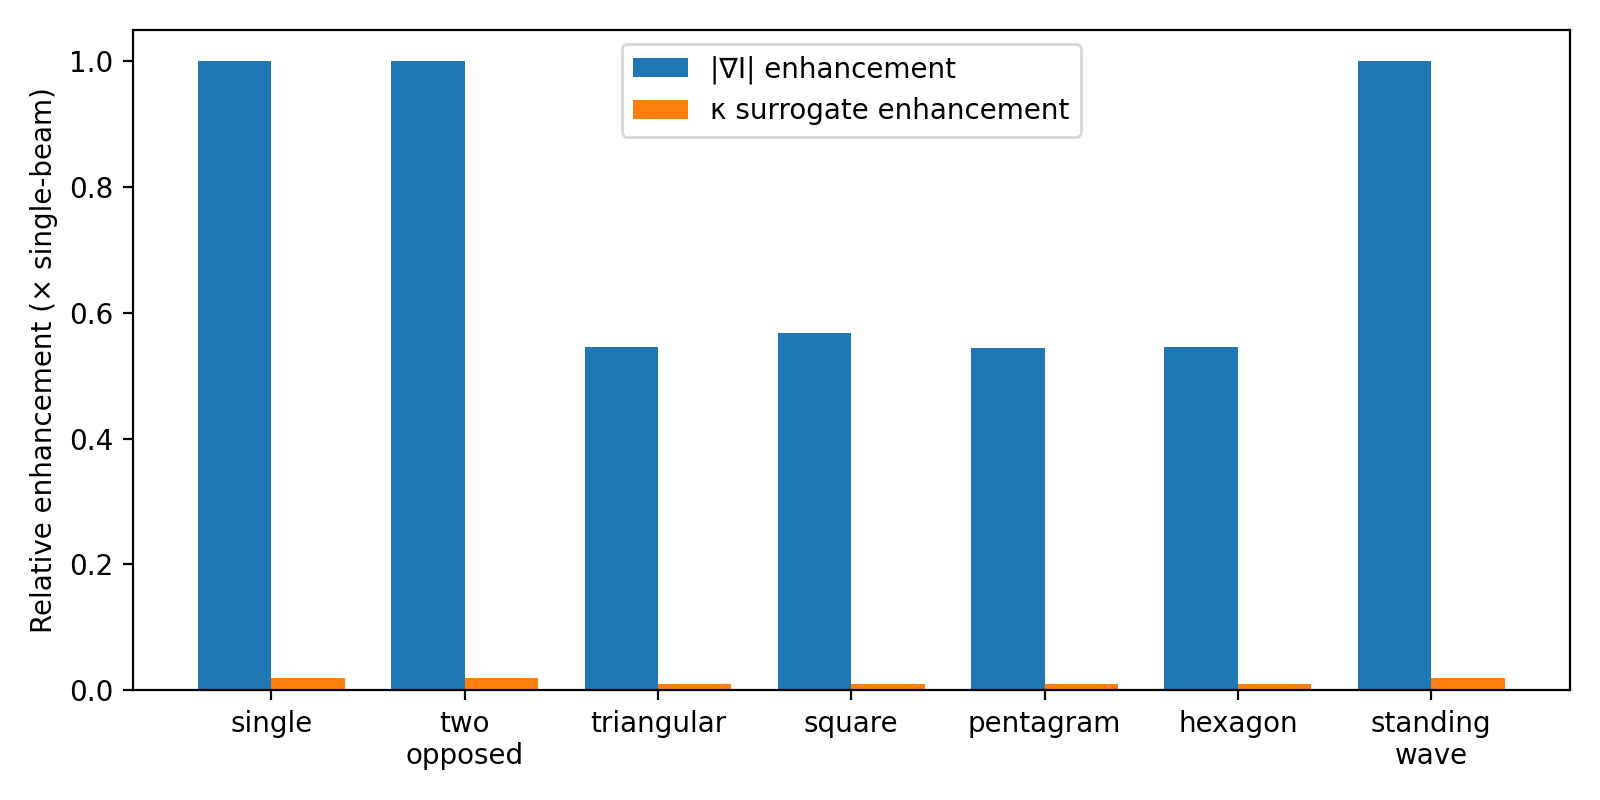
\includegraphics[width=0.8\linewidth]{figures/geometry_vs_kappa.png}
  \caption{Power-conserving envelope-scale geometry comparison. Bars show $|\nabla I|$ enhancement and a $\kappa$ surrogate; gains are modest near unity under fixed total power.}
\end{figure}

\begin{figure}[h]
  \centering
  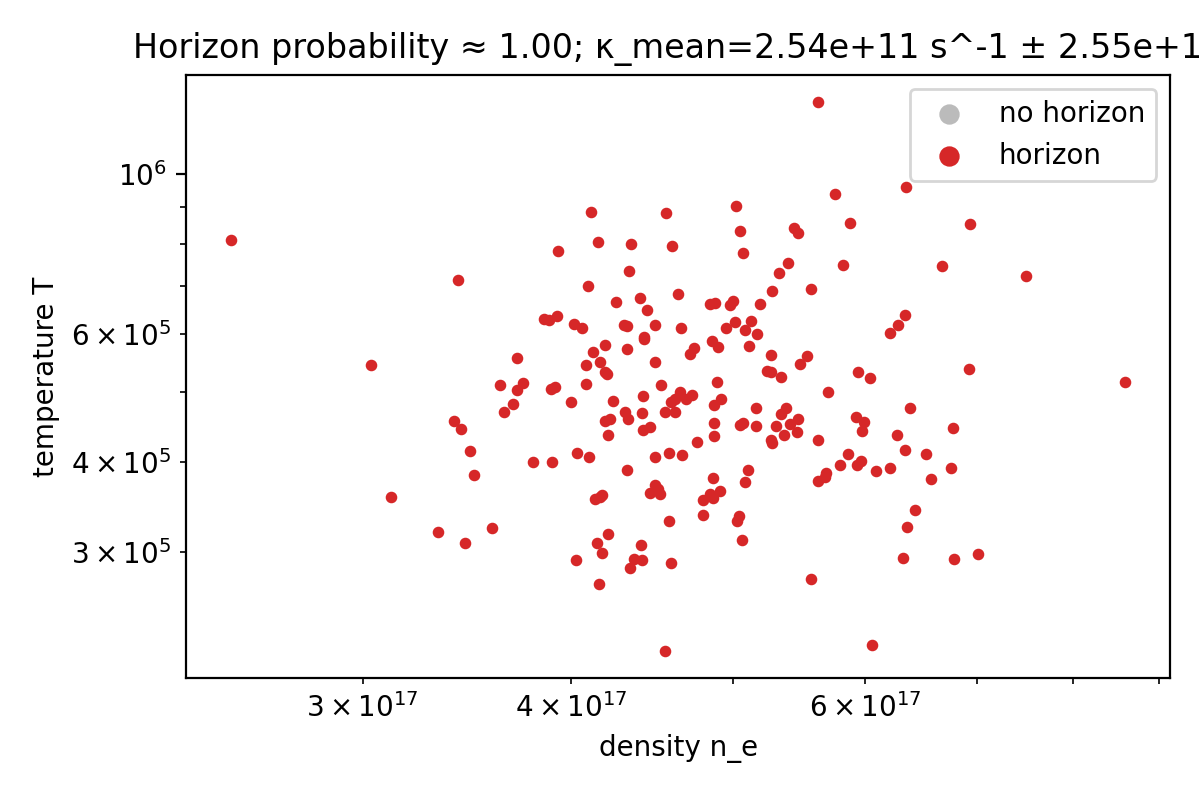
\includegraphics[width=0.75\linewidth]{figures/horizon_probability_bands.png}
  \caption{Uncertainty Monte Carlo: samples colored by horizon outcome with overall formation probability and $\kappa$ statistics.}
\end{figure}

\section{Discussion}
We achieved robust horizon formation with $\kappa\gg 10^{10}\,\mathrm{s^{-1}}$. PSD-based radio detectability is challenging for THz-peaked spectra \cite{Tonouchi2007}; the $T_H$ surrogate highlights potential feasibility pending normalization and coupling calibration. A radio-targeted sweep mode ($\kappa \sim 10^{10-11}\,\mathrm{s^{-1}}$) is provided to shift $T_H$ into radio and explore instrument trade-offs. By default our PSD normalization uses unit area and solid angle (or provided instrument parameters), so detectability scales directly with aperture, field of view, and coupling.

\paragraph{Limitations and future work.}
Our graybody fallback is a conservative proxy when profile-based transmission is unavailable; full wave calculations and measured optical coupling will refine normalization. Envelope-scale coarse graining neglects sub-structure that could modify $\kappa$ locally; end-to-end PIC/fluid coupling is a priority. Finally, instrument responses (bandpass, calibration) can be folded into $\eta$ and $\Omega$ to specialize the detectability maps to specific receivers.

\section{Code and Data}
Key scripts and modules are included as ancillary files:
\begin{itemize}
  \item \texttt{scripts/run\_param\_sweep.py}, \texttt{scripts/run\_full\_pipeline.py}
  \item \texttt{scripts/generate\_detection\_time\_heatmap.py}, \texttt{scripts/generate\_paramspace\_maps.py}
  \item \texttt{scripts/plot\_horizon\_profiles.py}, \texttt{scripts/hawking\_detection\_experiment.py}
  \item \texttt{src/analog\_hawking/physics\_engine/plasma\_models/fluid\_backend.py}
  \item \texttt{src/analog\_hawking/physics\_engine/plasma\_models/quantum\_field\_theory.py}
  \item \texttt{src/analog\_hawking/detection/radio\_snr.py}
\end{itemize}
See \texttt{results/} for sweep and validation JSON summaries.

\section*{Appendix: Reproducibility and Figure Generation}
All figures are generated from the version-controlled scripts in the repository root. Example commands:
\begin{verbatim}
# Set module path (if needed)
export PYTHONPATH="${PYTHONPATH}:src"

# Profile-derived graybody comparison (Figure: figures/graybody_impact.png)
python scripts/run_full_pipeline.py --demo

# Formation frontier and kappa at threshold
python scripts/compute_formation_frontier.py

# Geometry vs kappa surrogate (power-conserving)
python scripts/geometry_optimize_kappa.py

# Horizon probability bands under parameter uncertainty
python scripts/monte_carlo_horizon_uncertainty.py
\end{verbatim}
The \texttt{paper/} directory contains only the manuscript (\texttt{main.tex}), bibliography (\texttt{refs.bib}), and copied figures under \texttt{paper/figures/}. Source code lives exclusively under \texttt{scripts/} and \texttt{src/}.

\section*{Acknowledgments}
We thank collaborators and reviewers for insightful feedback.

\bibliographystyle{unsrt}
\bibliography{refs}

\end{document}
